\documentclass[11pt, a4paper]{article}
\usepackage[left=2cm, text={17cm, 24cm}, top=3cm]{geometry}
\usepackage[czech]{babel}
\usepackage[utf8]{inputenc}
\usepackage{times}
\usepackage{float}
\usepackage{enumitem}
\usepackage{multirow}
\usepackage{xcolor}
\usepackage{listings}

\lstset{basicstyle=\ttfamily,
  showstringspaces=false,
  commentstyle=\color{red},
  keywordstyle=\color{blue}
}

\usepackage{graphicx}
\usepackage{url}
\usepackage[nottoc,numbib]{tocbibind}

\lstset{
  columns=flexible,
  basicstyle=\small\ttfamily,
  mathescape=true,
  escapeinside=||
}

\begin{document}

\begin{titlepage}

\begin{center}
{\Huge \textsc{Vysoké učení technické v~Brně}\\[3mm]
\huge \textsc{Fakulta informačních technologií}}\\
\vspace{\stretch{0.382}}

{\LARGE Síťové aplikace a správa sítí\\[2mm]

\Huge Programování síťové služby\,--\,Analyzátor paketů}\\
\vspace{\stretch{0.618}}
\end{center}

{\Large \today \hfill Karel Ondřej}

\end{titlepage}

\tableofcontents

\newpage
\section{Uvedení do problematiky}

Cílem aplikace je offline analýza provozu na síti, který je uložen v několika souborech. Na každé vrstvě TCP/IP modelu se analyzují vybrané protokoly, které jsou popsány dále.

\subsection{Ethernet}

\begin{figure}[H]
  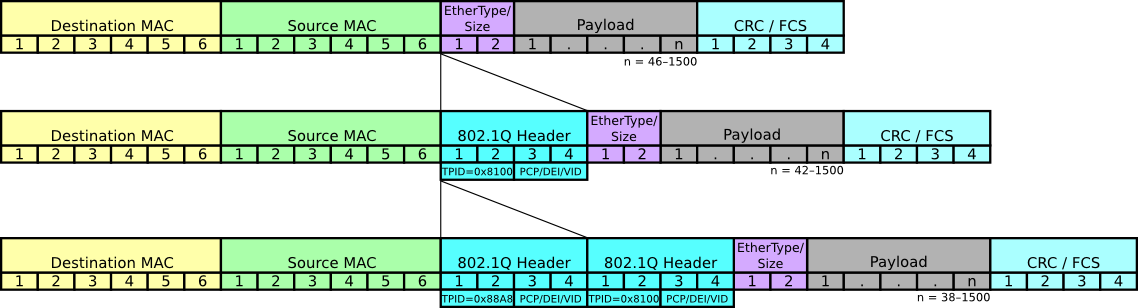
\includegraphics[width=\linewidth]{TCPIP_802_1ad_DoubleTag.png}
  \caption[]{Ethernet protokol včetně IEEE 802.1Q a IEEE 802.1ad\footnotemark}
  \label{fig:boat1}
\end{figure}
 \footnotetext{Zdroj: https://en.wikipedia.org/wiki/IEEE\_802.1ad}
Ethernet je protokol na vrstvě síťových rozhraní (L2), což je nejnižší vrstva TCP/IP modelu. Slouží k fyzickému spojení dvou zařízení za pomoci MAC adres. 
Pole EtherType v hlavičce určuje buď délku nebo typ protokolu přenášeného v obsahu. 
Pokud obsahuje hodnotu menší jak 1500, jedná se o délku obsahu, jinak se jedná o určení protokolu. 
\footnote{Zdroj: https://cs.wikipedia.org/wiki/Ethernet}

IEEE 802.1Q a IEEE 802.1ad jsou rozšíření Ethernetového rámce o VLAN. 
VLAN slouží k logickému rozdělení sítě nebo zařízení nezávisle na fyzické vrstvě. 
Jelikož oproti protokolu IP se jedná rozdělení už na vrstvě síťových rozhraní L2 místo podsítí na síťové vrstvě L3, lze usnadnit zprávu sítě, zvýšit výkon případně bezpečnost.

\begin{table}[h] \catcode`\-=12
	\centering
	\begin{tabular}{| l | l |}
		\hline
		EthernetType & Protokol\\ \hline
		0x0800 & IPv4 \\ \hline
		0x8100 & IEEE 802.1Q \\ \hline
		0x86DD & IPv6 \\ \hline
		0x88A8 & IEEE 802.1ad \\ \hline
	\end{tabular}
	\caption{Některé hodnoty EthernetType}
\end{table}

\subsection{IPv4}

Protokol IPv4 slouží k logickému směrování a rozdělení sítí. 
Směrování probíhá pomocí 4 bytových IP adres. 
Jedná se již o čtvrtou verzi IP protokolu, ale první rozšířenou tak, že v dnešní době je problém s nedostatkem adresního prostoru, díky jeho plýtvání, kdy byly přidělovány uživatelům rozsahy tak velké, že je nemohli nikdy využít. 
Z tohoto důvodu došlo k odebírání přebytečných adres, aby mohli být efektivněji využity.\footnote{Zdroj: https://cs.wikipedia.org/wiki/IPv4} 
Hlavička IPv4 je popsána v RFC 791. \cite{rfc:791}

\newpage
Důležité položky IPv4 hlavičky pro naší aplikaci:

\begin{figure}[h!]
\centering
  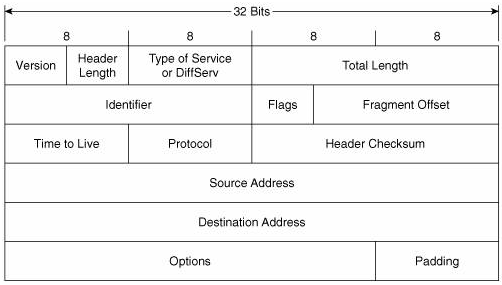
\includegraphics[width=0.6\linewidth]{ipv4-header.png}
  \caption[]{IPv4 hlavička\footnotemark}
\end{figure}
\footnotetext{Zdroj: https://advancedinternettechnologies.wordpress.com/ipv4-header/}
\begin{description}[style=multiline,leftmargin=3.5cm]
\item[IHL]
Určuje délku hlavičky v půl oktenu (4 bity), kdy nabývá nejméně hodnoty $5$, jelikož povinné parametry IPv4 hlavičky zabírají 20 bitů (5 půl oktenů). 
Určení celkové délky hlavičky lze tedy vyjádřit jako $(IHL*4)-1$.
\item[Identifikace]
Číslo, které identifikuje IP datagram. 
Tahle položka se použije v případě fragmentace datagramu, kdy s její pomocí a některých dalších položek, lze určit, který fragment patří ke kterému datagramu.
\item[Příznaky] 
Příznaky řízení fragmentace, kdy první bit je vždy 0. další bit se jmenuje \emph{Don’t fragment}, který zakazuje po cestě datagram fragmentovat. 
Poslední příznak \emph{More fragments} určuje, zda se jedná o poslední fragment (nastavený na 0) nebo jestli budou pokračovat další (hodnota 1).
\item[Offset fragmentu] 
Určuje začátek fragmentu v datagramu.
\item[TTL] 
\emph{Time to Live} zajišťuje, aby se datagram nezacyklil. 
Každý směrovač dekrementuje hodnotu TTL o jedna, pokud hodnota TTL dosáhne hodnoty nula je datagram zahozen. 
Jedná se o ekvivalent pro hop-limit u IPv6.
\item[Číslo protokolu] 
Určuje další protokol nacházející se za IP hlavičkou. 
Čísla jsou společná jak u IPv4 tak u IPv6.
\item[Zdrojová IP adresa] 
IP adresa reprezentující odesílatele.
\item[Cílová IP adresa] 
IP adresa reprezentující příjemce.
\end{description}

\begin{table}[H] \catcode`\-=12
	\centering
	\begin{tabular}{| l | l |}
		\hline
		Číslo protokolu & Protokol\\ \hline
		1  & ICMPv4 \\ \hline
		6  & TCP \\ \hline
		17 & UDP \\ \hline
		58 & ICMPv6 \\ \hline
	\end{tabular}
	\caption{Některé hodnoty čísla protokolu podstatné pro naši aplikaci (společné jak pro IPv4 tak IPv6).}
\end{table}

\subsection{IPv6}

Jedná se o další verzi protokolu IP, která oproti svému předchůdci rapidně zvětšuje adresový prostor ze 4 na 16 bytů. 
Dále odstraňuje kontrolní součet pro celý datagram, jelikož například položka TTL u IPv4 se při průchodem směrovačem měnila a celý součet se musel přepočítávat.

Nepovinné informace se v IPv6 předávají pomocí rozšiřujících hlaviček. 
Každá hlavička v poli \emph{next header} indikuje, která hlavička pokračuje. Poslední hlavička v řadě má číslo následujícího protokolu.\footnote{Zdroj: https://cs.wikipedia.org/wiki/IPv6}

\begin{figure}[h!]
\centering{}
  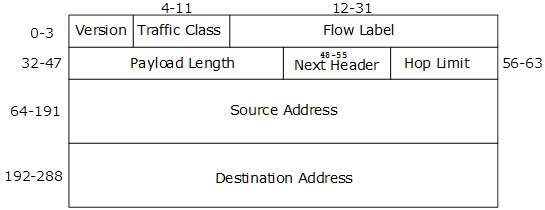
\includegraphics[width=0.6\linewidth]{IPv6_header.jpg}
  \caption[]{IPv6 hlavička\footnotemark}
\end{figure}
\begin{description}[style=multiline,leftmargin=3.5cm]

\item[Další hlavička] 
Udává následující rozšiřující hlavičku nebo protokol.
\item[Hop limit] 
Podobně jako u IPv4 TTL.
\item[Zdrojová IP adresa] 
16 bytová IP adresa reprezentující odesílatele.
\item[Cílová IP adresa] 
16 bytová IP adresa reprezentující příjemce.

\footnotetext{Zdroj: https://www.tutorialspoint.com/ipv6/ipv6\_headers.htm}
\end{description}

\begin{table}[h!] \catcode`\-=12
	\centering
	\begin{tabular}{| l | l |}
		\hline
		Kód další hlavičky & Další hlavička\\ \hline
		0 & Hop-by-Hop Options \\ \hline
		43 & Routing Header \\ \hline
		44 & Fragment Header \\ \hline
		60 & Destination Options \\ \hline
		135 & Mobility Header \\ \hline
		59 & No next header \\ \hline
	\end{tabular}
	\caption{Rozšiřující hlavičky důležité pro aplikaci.}
\end{table}

\subsection{ICMP}

Jedná se síťový protokol zapouzdřený v IP datagramu, sloužící k odesílání služebních informací nebo chybových hlášení jako nedostupnost zařízení nebo služby, přesměrování pokud existuje k cíli výhodnější cesta nebo vypršení časového limitu TTL (u IPv6 hop-limit). 
Verze ICMP pro IPv4 se označuje jako ICMPv4 a pro protokol IPv6 jako ICMPv6.\footnote{Zdroj: https://cs.wikipedia.org/wiki/ICMP} 

Jednotlivé zprávy jsou identifikované typem a dále blíže specifikované kódem. 
Podle typu zprávy  může obsahovat další doplňující informace, jako například původní IP hlavičku s začátkem dat. 
Bližší podrobnosti jsou specifikované pro ICMPv4 v RFC 792 a pro ICMPv6 v RFC 4443. \cite{rfc:792, rfc:4443}

Protokol ICMP používají také aplikace diagnostikující síť jako ping, který posílá zprávu \emph{Echo Request} a očekává vrácení \emph{Echo Reply}. 
Na základě toho rozhodne odezvu daného zařízení. 

\subsection{UDP}

UDP je protokolem na transportní vrstvě, který nedává žádnou záruku o doručení datagramu mezi uzly sítě. 
To znamená, že se můžou jednotlivé datagramy ztratit nebo můžou dojít opakovaně nebo v jiném pořadí. 
UDP jde tedy využít v aplikacích, kdy ztráta datagramu neznamená problém a klade se spíše důraz na jednoduchost jako například přenos hovoru. 
Protokol je popsán v RFC 768. \cite{rfc:768}

UDP slouží k propojení síťové vrstvy s aplikační, kdy lze na jeho základě určit aplikaci, které patří pře\-ná\-še\-né data. 
UDP hlavička se skládá ze čtyř 16 bitových položek, z toho jsou dvě povinná. 
Hlavička obsahuje položku zdrojový port (16 bitů), který není povinný, cílový port, který identifikuje aplikaci, které se mají předat data a proto je povinný, povinné políčko délka dat a volitelný kontrolní součet.

\subsection{TCP}

TCP je transportní protokol, který oproti protokolu UDP garantuje spolehlivý přenos zpráv tak, aby se žádná zpráva neztratila a všechny zprávy došli ve správném pořadí. 
Proto je také výrazně složitější a využívají ho aplikace, které potřebují navázat oboustranné spojení a nesmí docházet ke ztrátě dat. 
TCP protokol je podrobně popsán v RFC 793. \cite{rfc:793}

TCP stejně jako UDP slouží k propojení síťové vrstvy s aplikační vrstvou. 
Důležitými položkami TCP hlavičky pro naši aplikaci jsou: zdrojový port (16 bitů), cílový port (16 bitů), číslo sekvence (32 bitů), potvrzený bajt jinak ACK (32 bitů) a příznaky (6 bitů).
Zdrojový a cílový port identifikují stejně jako u UDP aplikaci, která data odeslala a která je má přijmout.
Číslo sekvence je pořadové číslo jednotlivých posílaných TCP sekvencí a ověřuje na straně příjemce jestli se sekvence neztratila a zda přišla ve správném pořadí.
Příjemce potom posílá zpět čísla správně přijatých sekvencí v poli potvrzený bajt.
Pokud odesílateli nedojde potvrzení v určitém intervalu, odešle pakety znovu.
Příznaky řídí celý přenos TCP sekvencí.

\section{Návrh aplikace}

\subsection{Řízení aplikace}

Prvním krokem aplikace je zpracování a ošetření parametrů z příkazové řádky. 
Dalším krokem je použití knihovny libcap pro práci se soubory ve formátu PCAP, obsahující uložené pakety. 
Knihovna se dokáže také postarat o filtraci jednotlivých paketů na základě výrazu. 
Následně se musí jednotlivé pakety ze všech souborů zpracovat. 
Pokud je požadovaná agregace nebo řazení, je daná operace provedena nad všemi pakety a následně jsou vypsány na standardní výstup.

\subsection{Analýza paketu}

Na začátku se uloží informace o samotném paketu jako pořadí, délka a časová značka. 
Následně se začne zpracovávat vrstva síťového rozhraní. 
V případě, že by paket obsahoval nepodporovaný protokol nebo by byl fragmentován a nelze zatím celý složit, dochází k zahození celého paketu a pořadí zůstane nezměněné. 
To znamená, že v případě zahození paketu číslo 5 bude číslo dalšího paketu opět 5, takže nedojde ve výstupním souboru k přeskakování pořadí čísel.

Na vrstvě síťového rozhraní je aplikací podporován pouze standardní protokol Ethernet včetně rozšíření hlavičky o VLAN (IEEE 802.1Q a IEEE 802.1ad). 
K paketu je přidán záznam, který uchovává informace o zdrojové a cílové MAC adrese, případně i hodnoty 802.1Q VLAN identifikátorů. 
Na základě položky typ v hlavičce se předá paket k zpracovávání síťové vrstvy. 
Pokud by typ neodpovídal protokolu IPv4 nebo IPv6, vypíše se na standardní chybový výstup chybová hláška, paket se zahodí a pokračuje se dalším paketem v pořadí.

Na síťové vrstvě jsou podporovány protokoly IPv4, IPv6, ICMPv4 a ICMPv6. 
V rámci návrhu se s protokoly ICMPv4 a ICMPv6 nakládá, jako by byli na vrstvě transportní. 
O protokolech IPv4 a IPv6 jsou ukládány informace o zdrojové IP adrese, cílové IP adrese a TTL (hop-limit).

U protokolu IPv4 je podporována možnost fragmentace paketu. 
K tomu lze použít algoritmus z RFC 815, který slouží k určení, zda už přišel celý paket a následně je ho možné složit a předat k další analýze. \cite{rfc:815}
Které fragmenty patří ke kterému paketu lze určit čtveřicí hodnot z hlavičky: zdrojová IP adresa, cílová IP adresa, identifikátor a číslo protokolu. 

Samotný algoritmus pro sestavení fragmentu je velmi jednoduchý. 
Při příchodu prvního fragmentu se vytvoří množina děr (díra reprezentuje chybějící část paketu), která bude obsahovat díru $<0; \infty>$. 
Místo nekonečna může být použito velmi velké číslo.
Následně se prochází množinou děr a hledá se díra, kterou by příchozí fragment vyplnil. 
Když taková díra existuje, odstraní se z množiny. 
Pokud fragment nezaplní celou díru, přidají se do množiny díry od počátku odstraněné díry do začátku fragmentu a v případě, že fragment není poslední, se přidá díra od konce fragmentu do konce díry. 
Když je množina děr prázdná, byli obdrženy všechny fragmenty a může se složit kompletní paket.
Po složení dat se do paketu uloží informace o zdrojové a cílové IP adrese a TTL z posledního příchozího paketu a data se předají k zpracování transportní vrstvy.

V případě IPv6 protokolu se z hlavičky uchovávají informace o cílové IP adrese, zdrojové IP adrese a hop-limit. 
Následně se podívá na typ dalšího protokolu nebo rozšiřující hlavičky. 
Pokud se jedná o transportní protokol nebo ICMPv6, předá se zpracování transportní vrstvy. 
V případě rozšiřujících hlaviček se zpracují a zjistí další typ hlavičky, dokud se nebude jednat o transportní protokol nebo ICMPv6. 
V případě naražení na typ indikující, že už nepokračuje žádná další hlavička ani protokol, případně rozšiřující hlavičky AH a ESP, které nejsou podporované, vypíše se na standardní chybový výstup hláška a paket se zahodí. 
To samé platí o nepodporovaných protokolech transportní vrstvy.

Na transportní vrstvě jsou podporovány protokoly UDP a TCP. 
V případě jiného protokolu je paket zahozen a je vypsána chybová hláška na standardní chybový výstup a pokračuje se zpracováním dalšího paketu. 
U obou protokolů se uchovává informace o zdrojovém a cílovém portu a v případě TCP navíc číslo sekvence (sequence number), potvrzený bajt (acknowledgment number) a příznaky.

I když ICMPv4 a ICMPv6 se nachází na síťové vrstvě, je s nimi v aplikaci nakládáno jako kdyby byli na vrstvě transportní. 
Zjednodušuje to návrh, kdy paket vždy obsahuje z každé ze tří vrstev jeden protokol. 
U obou protokolů se uchovají informace o typu a kódu zprávy.

\subsection{Řazení a agregace}

Agregace jednotlivých paketů se provádí na základě zdrojové a cílové MAC adresy, IP adresy a portů, až po zpracování všech souborů. 
Pakety jsou nejdříve analyzovány a potom jsou po jednom procházeny a z každého je zjištěna hodnota, podle které se agreguje. 
Pokud ještě neexistuje skupina, která by reprezentovala skupinu kam daný paket patří, je daná skupina vytvořena.
Paket je poté vložen do skupiny, kam na základě agregace patří. 
Pořadí agregovaných skupin v případě agregace bez seřazení závisí na pořadí vytvoření jednotlivých skupin. 
To znamená, že pořadí skupin bude podléhat prvnímu výskytu paketu spadajícího do skupiny v souboru.

Samotné řazení je buď prováděno nad agregovanými skupinami nebo nad pakety na základě klíče, který může být velikost nebo počet paketů. 
V případě agregace se bere součet velikosti všech paketů ve skupině nebo jejich počet. 
Řazení podle počtu paketů nad jednotlivými pakety nemá žádný efekt, jelikož počet paketů je vždy roven 1. 
Samotné řazení je stabilní, takže v případě shodných hodnot zůstanou pakety v pořadí, v jakém jsou uloženy v souborech (paket, který přišel později bude na výstupu níže).

\section{Implementace}

Aplikace je implementovaná v jazyce C/C++ s použitím knihovny libpac pro offline zpracovávání paketů ze souboru.

\subsection{Uchovávání informací o paketu}

Analýza paketu je implementovaná pomocí třídy \texttt{Parser}, která taky pakety agreguje a řadí. Jednotlivé protokoly reprezentují třídy \texttt{Ethernet}, \texttt{IPv4}, \texttt{IPv6}, \texttt{ICMPv4}, \texttt{ICMPv6}, \texttt{UDP} a \texttt{TCP}. 

Každá třída uchovává potřebné informace o daném protokolu v původní struktuře podle použité hlavičky (např. pro \texttt{IPv4} jsou IP adresy uloženy ve struktuře in\_addr a TTL jako uint8\_t), jelikož se jedná o efektivní uložení v paměti. Dále třídy obsahují metodu \texttt{toString}, která vrací textovou reprezentaci daného protokolu (např. pro třídu \texttt{Ethernet} metoda \texttt{toString} vrací řetězec Ethernet: 50:e5:49:3d:8c:43 ff:ff:ff:ff:ff:ff) a podle vrstvy na které se daný protokol nachází, metody vracející MAC adresu, IP adresu nebo port jako řetězec, potřebný pro agregaci (např. třída \texttt{Ethernet} obsahuje metody \texttt{srcMac} a \texttt{dstMac}). Protokoly ICMP jsou pro jednoduchost implementované jako protokoly transportní vrstvy, kdy metody pro vrácení zdrojového a cílového portu vrací prázdný řetězec. To se dále využívá u agregace, kdy se všechny pakety vracející prázdný řetězec neagregují. 

Jednotlivé pakety v souborech reprezentuje třída \texttt{Packet}, která uchovává informace o pořadí paketu, časovou značku, délku paketu a protokoly L2, L3 a L4 vrstvy v podobě dříve zmiňovaných tříd. Také obsahuje metodu pro získání délky, potřebnou pro řazení, metody pro získání zdrojových a cílových MAC adres, IP adres a portů uložených protokolů a metodu \texttt{toString}, která se stará o textovou reprezentaci celého paketu.

\subsection{Fragmentace IPv4}

O sestavení fragmentovaného paketu se stará třída \texttt{Parser}. Jednotlivé fragmenty a díry jsou uloženy ve dvou asociativních polích typu \texttt{map}, kde jako klíč slouží třída \texttt{Parser::FragmentKey}, které obsahují vektory třídy \texttt{Parser::Fragment}. \texttt{Parser::FragmentKey} obsahuje položky reprezentující zdrojovou a cílovou IP adresu jako strukturu in\_addr, identifikátor fragmentu jako uint8\_t a číslo protokolu jako uint8\_t, které jsou vhodné pro následné porovnání. Třída také přetěžuje operátory $==$ a $<$, aby šla použít jako klíč do asociativního pole. Jednotlivé fragmenty a díry reprezentuje třída \texttt{Parser::Fragment}, která ukládá pozici prvního a posledního bytu ve fragmentu. Pokud se jedná o fragment obsahuje také data.

Po provedení algoritmu viz návrh, se začnou sestavovat jednotlivé fragmenty dohromady. V pří\-pa\-dě pří\-cho\-zí\-ho fragmentu, který z části překrývá jiný a z části zaplňuje díru v paketu, se při sestavování použijí data pro překrývající část z pos\-led\-ní\-ho pří\-cho\-zí\-ho paketu. Výsledný sestavený paket obsahuje časovou značku a velikost podle posledního příchozího paketu.

\subsection{Agregace a řazení}

Agregace probíhá až po zpracování všech paketů. Jednotlivé agregované položky jsou reprezentovány strukturou \texttt{Parser::Group}, která obsahuje položky key (jedná se o MAC adresu, IP adresu nebo port podle parametru agregace), length pro celkovou délku všech podobných paketů a count pro jejich počet. Položka key je řetězec, jelikož je jednoduché na něj převést všechny zmiňované položky a dále jde jednoduše porovnávat. Při agregaci se třídě \texttt{Parser} předá parametr, podle kterého se má agregovat. Následně se prochází vektor všech paketů a zavolá se na něm metoda odpovídající zadanému klíčí. Dále se projde vektorem všech agregovaných položek a pokud už existuje skupina, kam paket spadá, je jeho velikost přičtena k celkové velikosti a počet inkrementován o jedna, jinak je vytvořena. Pokud metoda vrátí prázdný řetězec, je daný paket vynechán. Jedná se o agregaci podle zdrojového a cílového portu nad paketem obsahující protokol ICMP.

Pro řazení byla implementovaná třída \texttt{Parser::Sort}, které se předá parametr, podle kterého se má řa\-dit. Také obsahuje pravidla pro řazení tříd \texttt{Parser::Packet} a \texttt{Parser::Group} na základě zadaného klíče. O~samotné řa\-ze\-ní se sta\-rá funk\-ce \texttt{stable\_sort} z STL knihovny algorithm, která vy\-u\-ží\-vá jako klíč pro řazení třídu \texttt{Parser::Sort}.

\newpage

\section{Informace o programu}

Program slouží k offline analýze síťového provozu uloženého v souboru formátu PCAP. 
Aplikace podporuje rodinu protokolů TCP/IP a to na L2 vrstvě protokol Ethernet, na L3 vrstvě protokoly IPv4, IPv6, ICMPv4 a ICMPv6, na L4 vrstvě UDP s TCP protokolem. 
Vrstva L7 se neanalyzuje.

\subsection{Použití}

isashark [-h] [-a aggr-key] [-s sort-key] [-l limit] [-f filter-expression] file ...

\begin{description}[style=multiline,leftmargin=3.5cm]

\item[-h] Vypíše nápovědu na standardní výstup a ukončí program.
\item[-a aggr-key] Seskupí pakety do skupin podle zadaného kritéria a určí jejich celkovou velikost a počet. Klíč \emph{aggr-key} může nabývat hodnot \emph{srcmac} pro zdrojovou MAC adresu, \emph{dstmac} pro cílovou adresu, \emph{srcip} pro zdrojovou IP adresu, \emph{dstip} pro cílovou IP adresu, \emph{srcport} pro zdrojový port a \emph{dstport} pro cílový port. V případě použití \emph{srcport} a \emph{dstport} se protokoly ICMP nebudou agregovat.
\item[-s sort-key] Seřazení paketů nebo agregovaných skupin podle klíče \emph{sort-key}. Hodnoty \emph{sort-key} mů\-žou být \emph{bytes} pro seřazení podle velikosti nebo \emph{pakets} pro seřazení podle počtu paketů. Seřazení paketů podle klíče \emph{pakets} nebude mít žádný vliv.
\item[-l limit] Vypíše první položky až do hodnoty limitu.
\item[-f filter-expression] Pakety budou vyfiltrovány na základě zadaného výrazu.
\item[file] Jednotlivé soubory formátu PCAP obsahující záznam provozu na síti.

\end{description}

\subsection{Příklady}

\begin{enumerate}
\item Seskupení paketů podle cílové MAC adresy bez řazení.

\begin{lstlisting}[language=bash]
./isashark -a srcmac file.pcap
\end{lstlisting}

\item Seskupení paketů podle zdrojového portu a seřazení podle počtu paketů ze zadaných souborů.

\begin{lstlisting}[language=bash]
./isashark -a dstport -s pakets file01.pcap file02.pcap file03.pcap 
\end{lstlisting}

\item Program analyzuje zadaný soubor, z kterého vyfiltruje všechny pakety s cílovou IP adresou 192.168.56.1.

\begin{lstlisting}[language=bash]
./isashark -f "dst host 192.168.56.1" file.pcap 
\end{lstlisting}

\item Vypsání prvních 10 paketů seřazených podle velikosti.

\begin{lstlisting}[language=bash]
./isashark -l 10 -s bytes file.pcap 
\end{lstlisting}

\end{enumerate}
\newpage
\def\refname{Literatura}
\bibliographystyle{czechiso}
\bibliography{manual}
\nocite{rfc:2460}
\end{document}